\section{系统实现}

\subsection{前台页面实现}

\subsubsection{首页页面实现}

进入到智慧工厂管理系统的首页,首先向客户或者供应商展示公司介绍,第一个页面有公司标语和简短介绍等;在上方的导航栏有一些功能按钮,例如工厂特点介绍、提供的服务、工厂的特点、联系方式和管理员登录入口等,系统的前台展示如图\ref{fig:index}所示。

\begin{figure}[H]
    \centering
    \begin{subfigure}{.45\textwidth}
        \centering
        
\includegraphics[width=\textwidth]{figures/5index.png}
        \subcaption{系统首页展示图}
        \label{fig:index1}
    \end{subfigure}
    \qquad
    \begin{subfigure}{.45\textwidth}
        \centering
        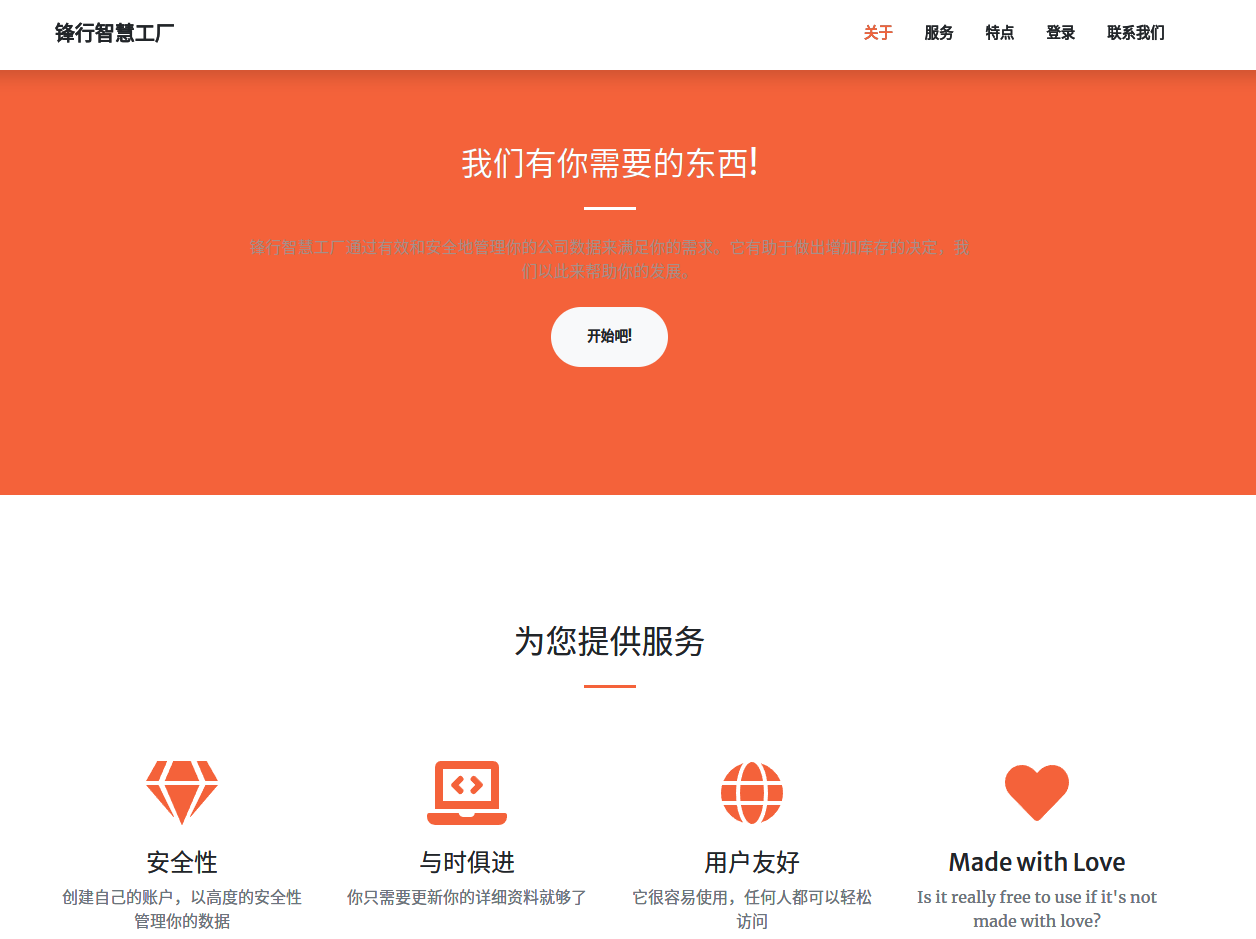
\includegraphics[width=\textwidth]{figures/5index2.png}
        \subcaption{工厂服务特点图}
        \label{fig:index2}
    \end{subfigure}
    \\
    \begin{subfigure}{.45\textwidth}
        \centering
        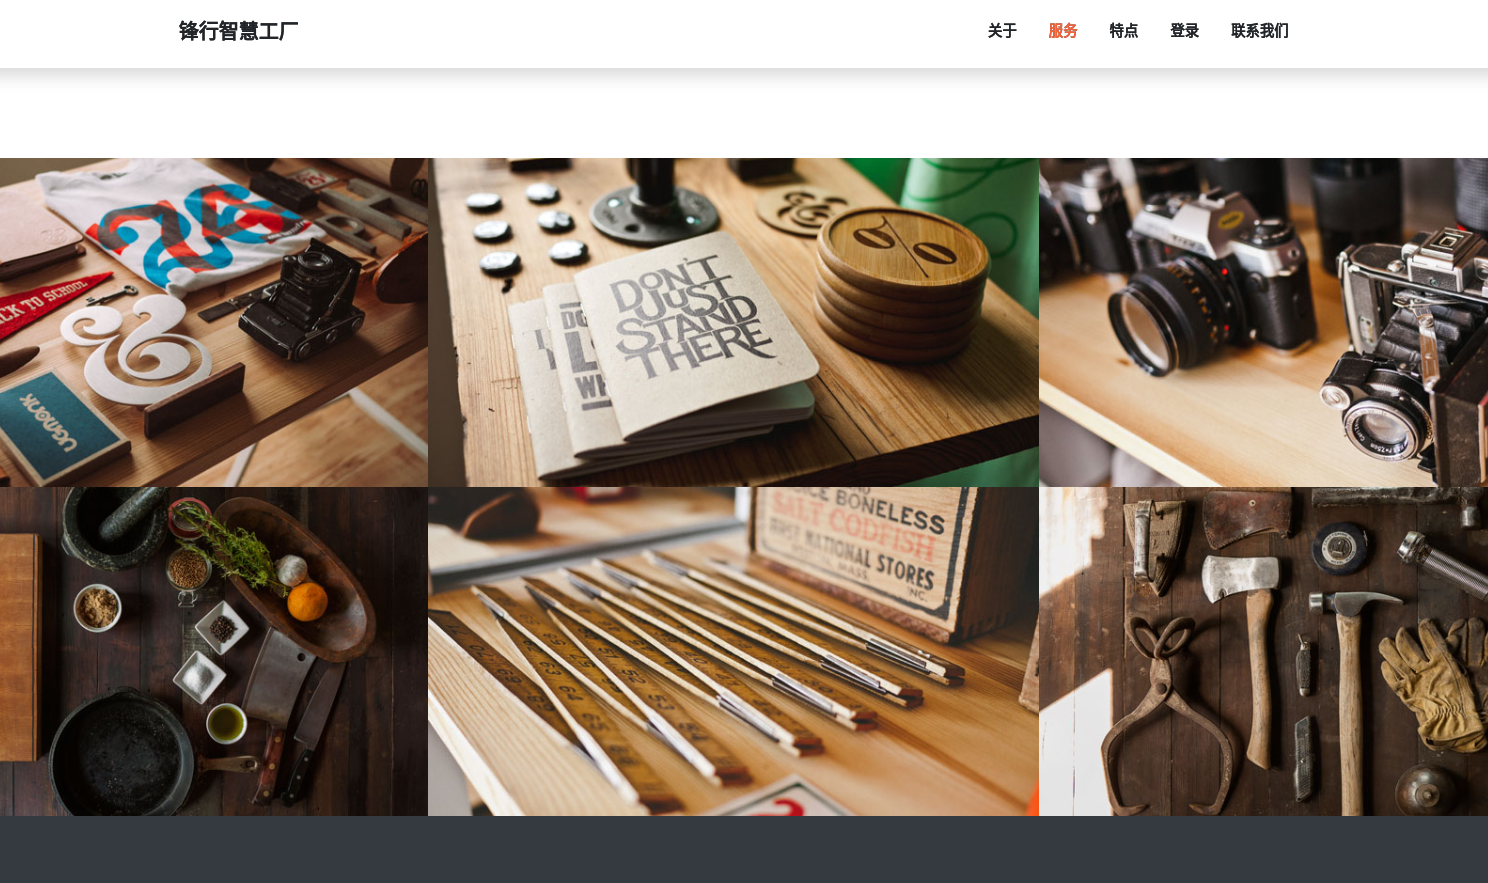
\includegraphics[width=\textwidth]{figures/5index3.png}
        \subcaption{工厂介绍图片页面图}
        \label{fig:index3}
    \end{subfigure}
    \qquad
    \begin{subfigure}{.45\textwidth}
        \centering
        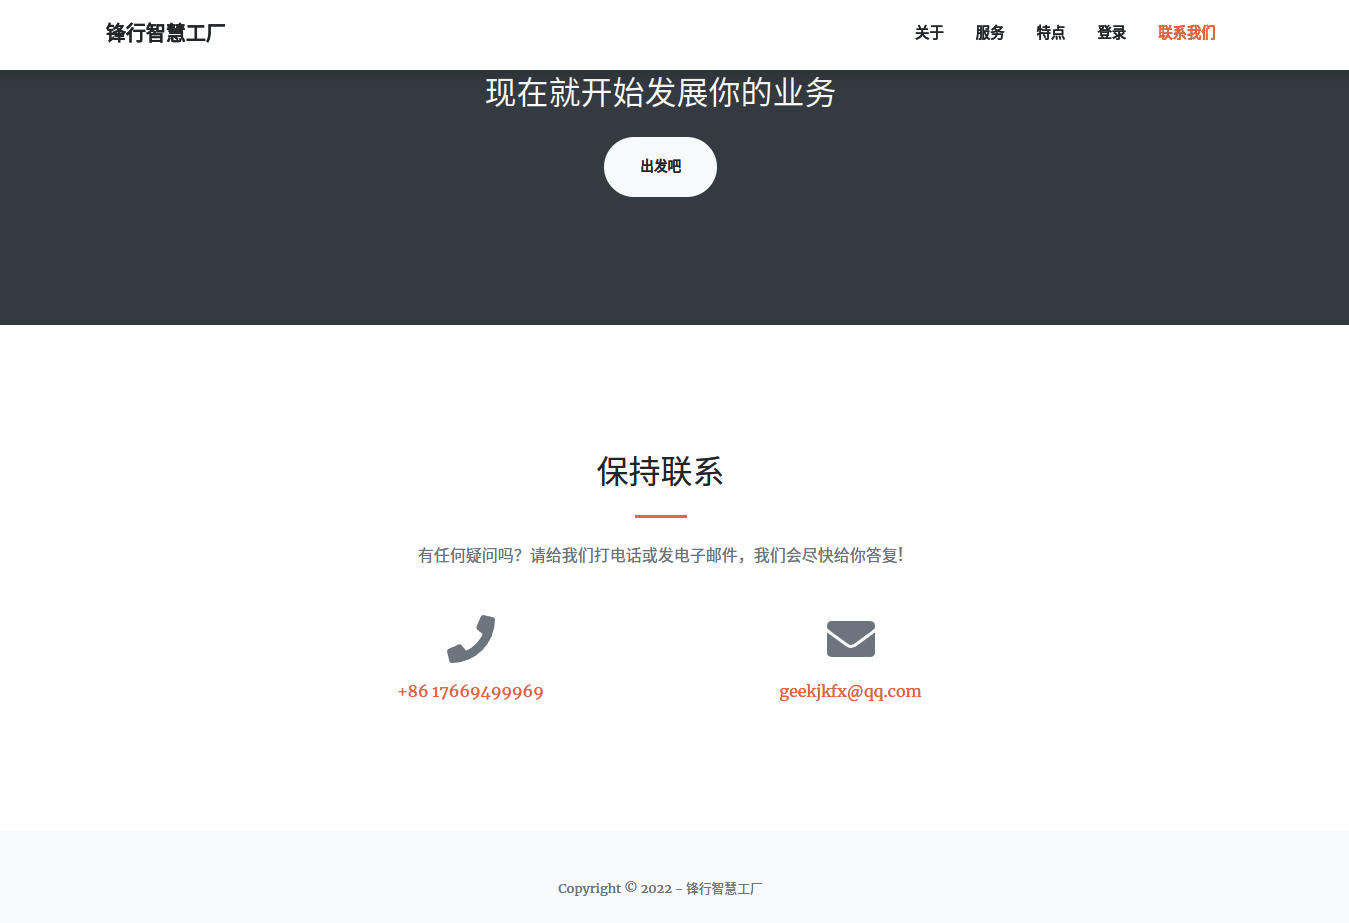
\includegraphics[width=\textwidth]{figures/5index4.png}
        \subcaption{工厂联系方式页面图}
        \label{fig:index4}
    \end{subfigure}
    \caption{前台页面展示图}
    \label{fig:index}
\end{figure}

如图\ref{fig:index1}所示,通过首页页面向客户展示工厂标语以及服务介绍;如图\ref{fig:index2}所示,向客户进一步介绍工厂服务内容以及服务特点情况;如图\ref{fig:index3}所示,向客户展示工厂生成环境图片,当鼠标移到图片上可进一步显示图片内容介绍;如图\ref{fig:index4}所示,最后向客户提供工厂的联系方式等信息。

\subsubsection{登录注册页面实现}

系统首页除展示完工厂介绍之外,在上方导航栏位置处还有登录按钮供工厂管理人员对工厂信息进行管理入口。如图\ref{fig:loginpage}所示,在后台登录页面,管理人员输入管理账号与密码进行登录。如图\ref{fig:register}所示,工厂的某一个部门组织可以在注册页面注册管理账号,并且填写组织名称、电子邮件、电话号码、登录用户名以及密码等信息。

\begin{figure}[H]
    \centering
    \begin{subfigure}{.45\textwidth}
        \centering
        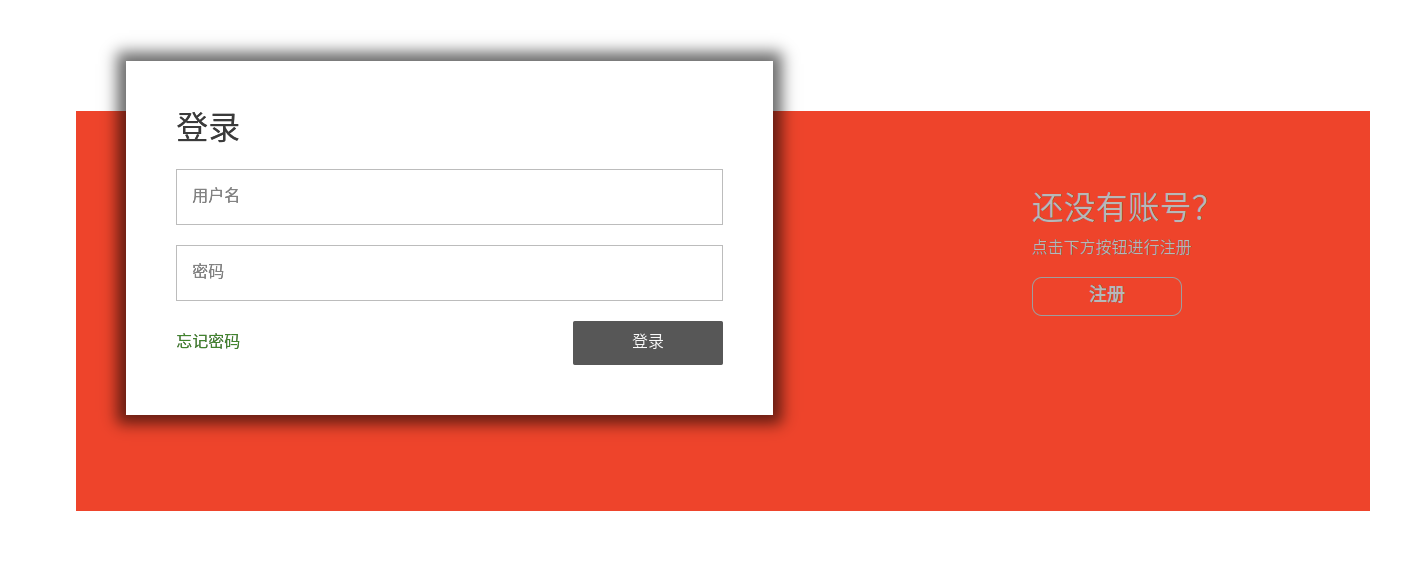
\includegraphics[width=\textwidth]{figures/5login.png}
        \subcaption{登录页面图}
        \label{fig:loginpage}
    \end{subfigure}
    \qquad
    \begin{subfigure}{.45\textwidth}
        \centering
        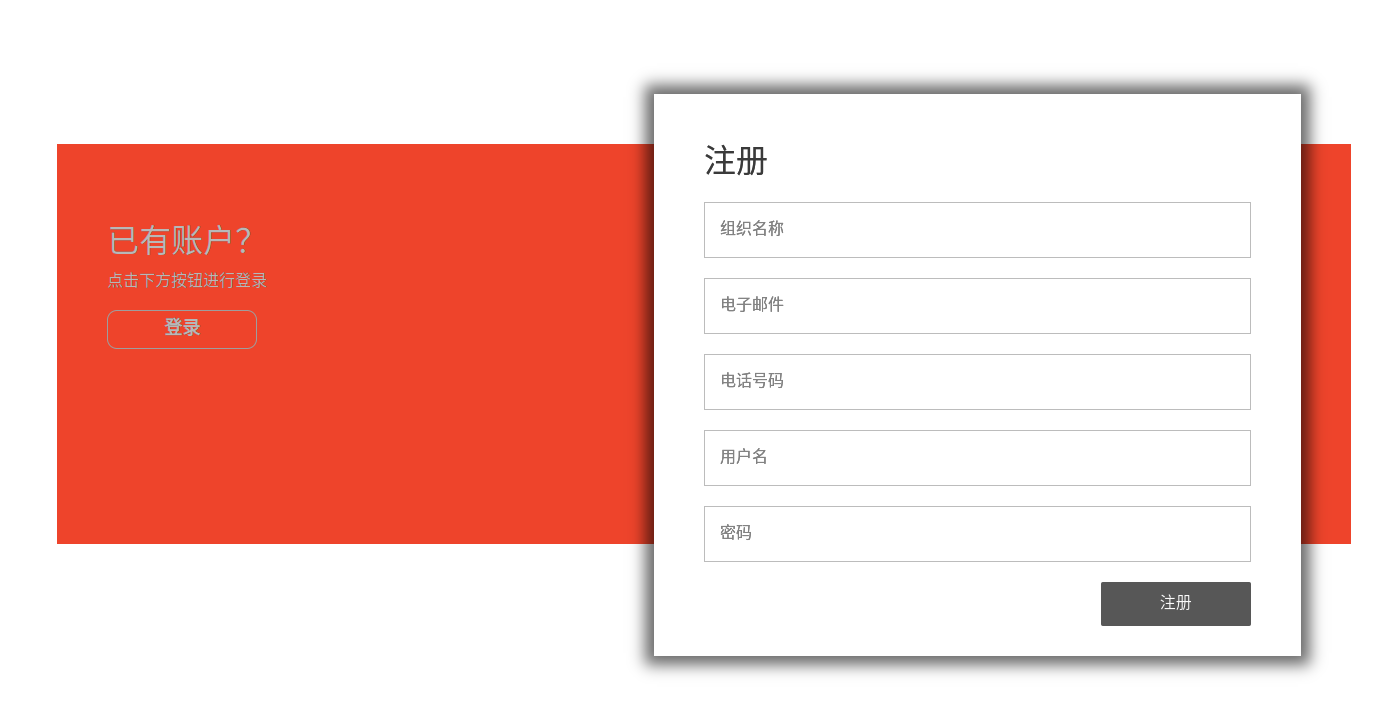
\includegraphics[width=\textwidth]{figures/5register.png}
        \subcaption{注册页面图}
        \label{fig:register}
    \end{subfigure}
    \caption{登录注册页面图}
\end{figure}

\subsection{后台页面实现}

\subsubsection{后台管理仪表盘页面实现}

当工厂部门组织管理员登录到后台管理页面,首先向管理员展示仪表盘页面,该仪表盘可以从工厂各个角度展示工厂当前部门组织的交易情况。

\begin{figure}[H]
    \centering
    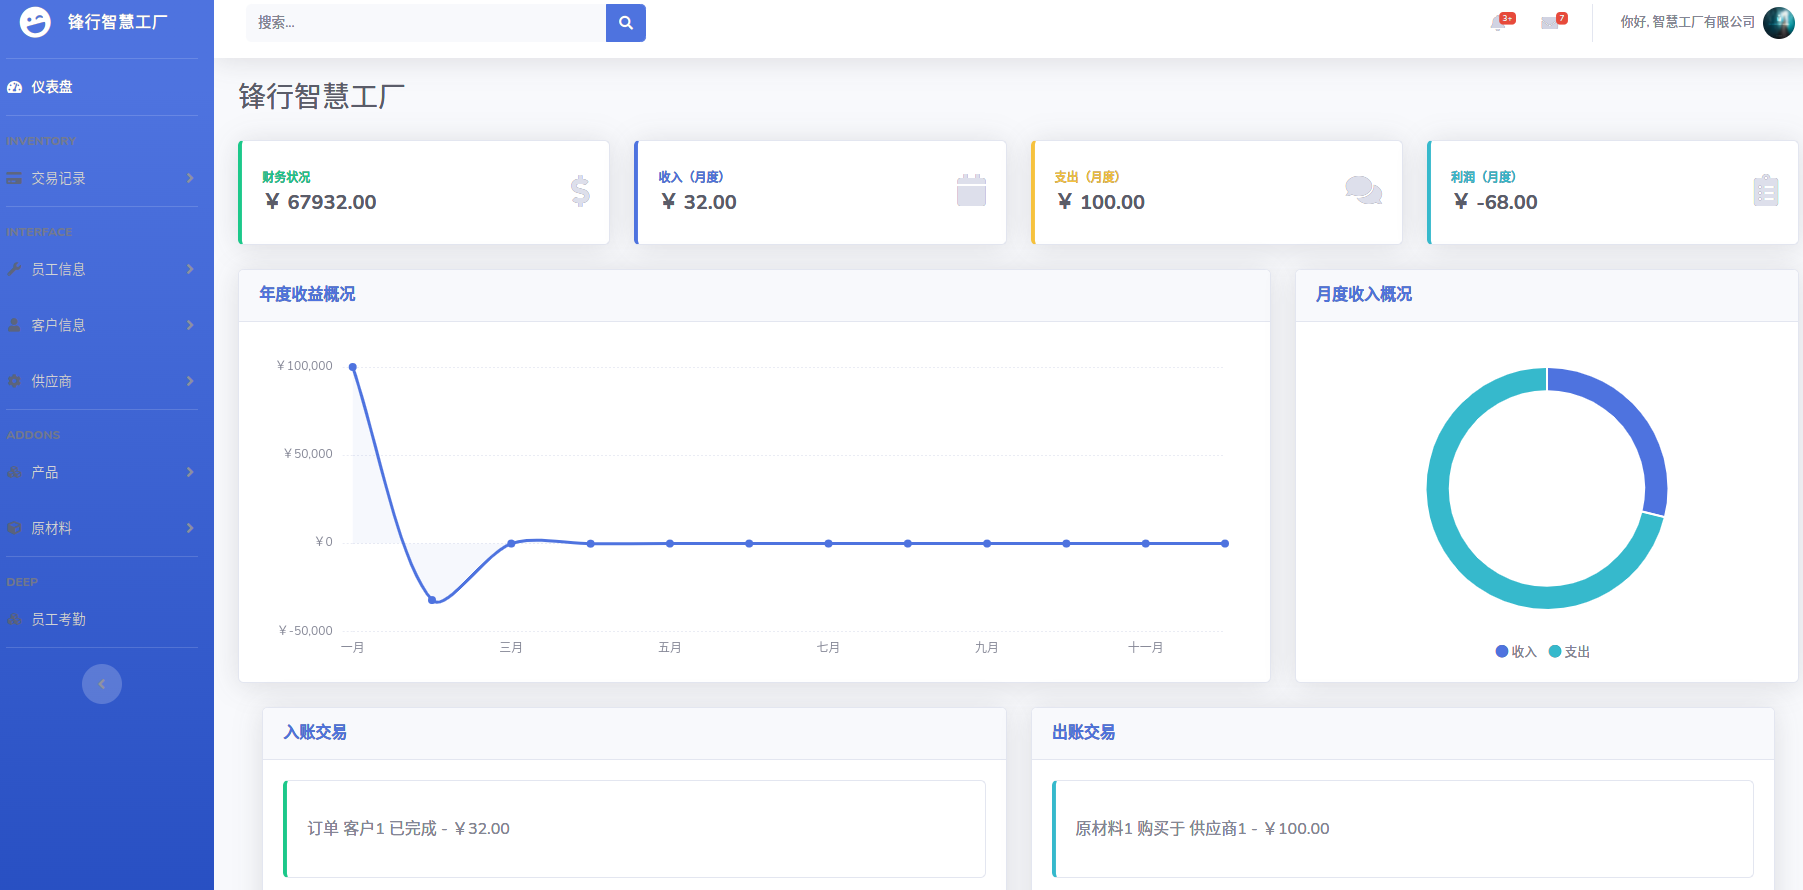
\includegraphics[width=.75\textwidth]{figures/5dashboard.png}
    \caption{后台仪表盘页面图}
    \label{fig:dashboard}
\end{figure}

如图\ref{fig:dashboard}所示,后台首页页面左方一栏是后台管理功能导航栏;右上方为当前登录部门组织账号概览;仪表盘页面第一行为当前组织部门财务状况的数字展示,其中包括财务状况和月度的收入、支出以及利润信息;第二行为当前组织部门的财务状况的可视化展示,包括年度收入支出的折线图以及月度收入支出的饼图;在最下方,向管理员展示最近的交易记录,左部分展示入账的交易记录,右方展示出账的交易记录。

\subsubsection{后台信息管理功能实现}

在工厂管理员进入到后台管理页面之后,在左方的导航栏处排列了各种工厂信息管理的页面按钮。如图\ref{fig:dashboard}所示,其中包括交易记录、员工信息、客户信息、供应商信息、产品信息、原材料信息和员工考勤按钮,点击特定导航栏按钮,可以展开二级菜单展示当前信息管理的各种操作。

% \begin{figure}[H]
%     \centering
%     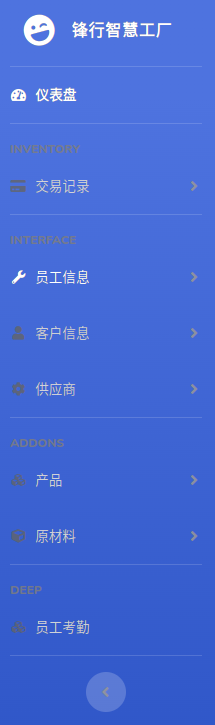
\includegraphics[width=.2\textwidth]{figures/5navigationbar.png}
%     \caption{后台导航栏图}
%     \label{fig:navigation}
% \end{figure}

点击特定导航栏按钮之后展开的人员管理类的信息管理操作;如图\ref{fig:employee}所示,展示了员工信息的信息管理操作,其中包括查看员工、添加员工以及支付薪资按钮操作;如图\ref{fig:customer}所示,展示客户信息的管理操作;如图\ref{fig:suplier}所示,展示了供应商信息的管理操作。

\begin{figure}[H]
    \centering
    \begin{subfigure}{.25\textwidth}
        \centering
        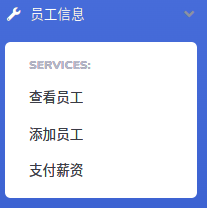
\includegraphics[width=\textwidth]{figures/5employee.png}
        \subcaption{员工信息二级菜单图}
        \label{fig:employee}
    \end{subfigure}
    \qquad
    \begin{subfigure}{.25\textwidth}
        \centering
        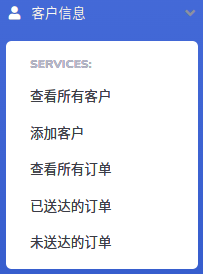
\includegraphics[width=\textwidth]{figures/5customer.png}
        \subcaption{客户信息二级菜单图}
        \label{fig:customer}
    \end{subfigure}
    \qquad
    \begin{subfigure}{.25\textwidth}
        \centering
        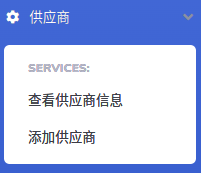
\includegraphics[width=\textwidth]{figures/5supplyer.png}
        \subcaption{供应商信息二级菜单图}
        \label{fig:suplier}
    \end{subfigure}
    \caption{人员管理类信息管理菜单图}
\end{figure}

点击特定导航栏按钮之后展开的产品与原材料的信息管理操作;如图\ref{fig:product}所示,展示了产品信息的信息管理操作,其中包括查看所有产品以及添加产品操作;如图\ref{fig:raw}所示,展示原材料信息的管理操作。

\begin{figure}[H]
    \centering
    \begin{subfigure}{.25\textwidth}
        \centering
        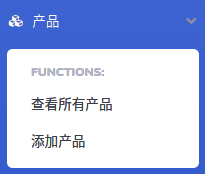
\includegraphics[width=\textwidth]{figures/5product.png}
        \subcaption{产品信息二级菜单图}
        \label{fig:product}
    \end{subfigure}
    \qquad
    \begin{subfigure}{.25\textwidth}
        \centering
        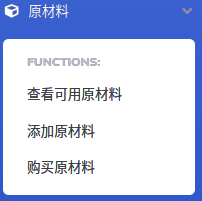
\includegraphics[width=\textwidth]{figures/5raw.png}
        \subcaption{原材料信息二级菜单图}
        \label{fig:raw}
    \end{subfigure}
    \caption{产品、原材料信息管理菜单图}
\end{figure}

在人员信息管理方面,管理员可以在后台页面查看当前工厂的人员信息内容,内容以表格的形式呈现,如图\ref{fig:empledtl}所示,管理员可以查看当前工厂员工信息表格,并且在此页面可以对员工进行支付薪资、下达工作任务以及删除员工等操作,并且在页面右下方还有计算工资以及添加员工的快捷按钮;如图\ref{fig:cstmdtl}所示,向管理员展示客户信息表格,并且可以通过表格超链接按钮对指定客户进行下单操作以及查看指定客户的订单详情;如图\ref{fig:spledtl}所示,向管理员展示供应商信息表格;如图\ref{fig:prdctdtl}所示,向管理员展示产品信息详情表格。

\begin{figure}[H]
    \centering
    \begin{subfigure}{.45\textwidth}
        \centering
        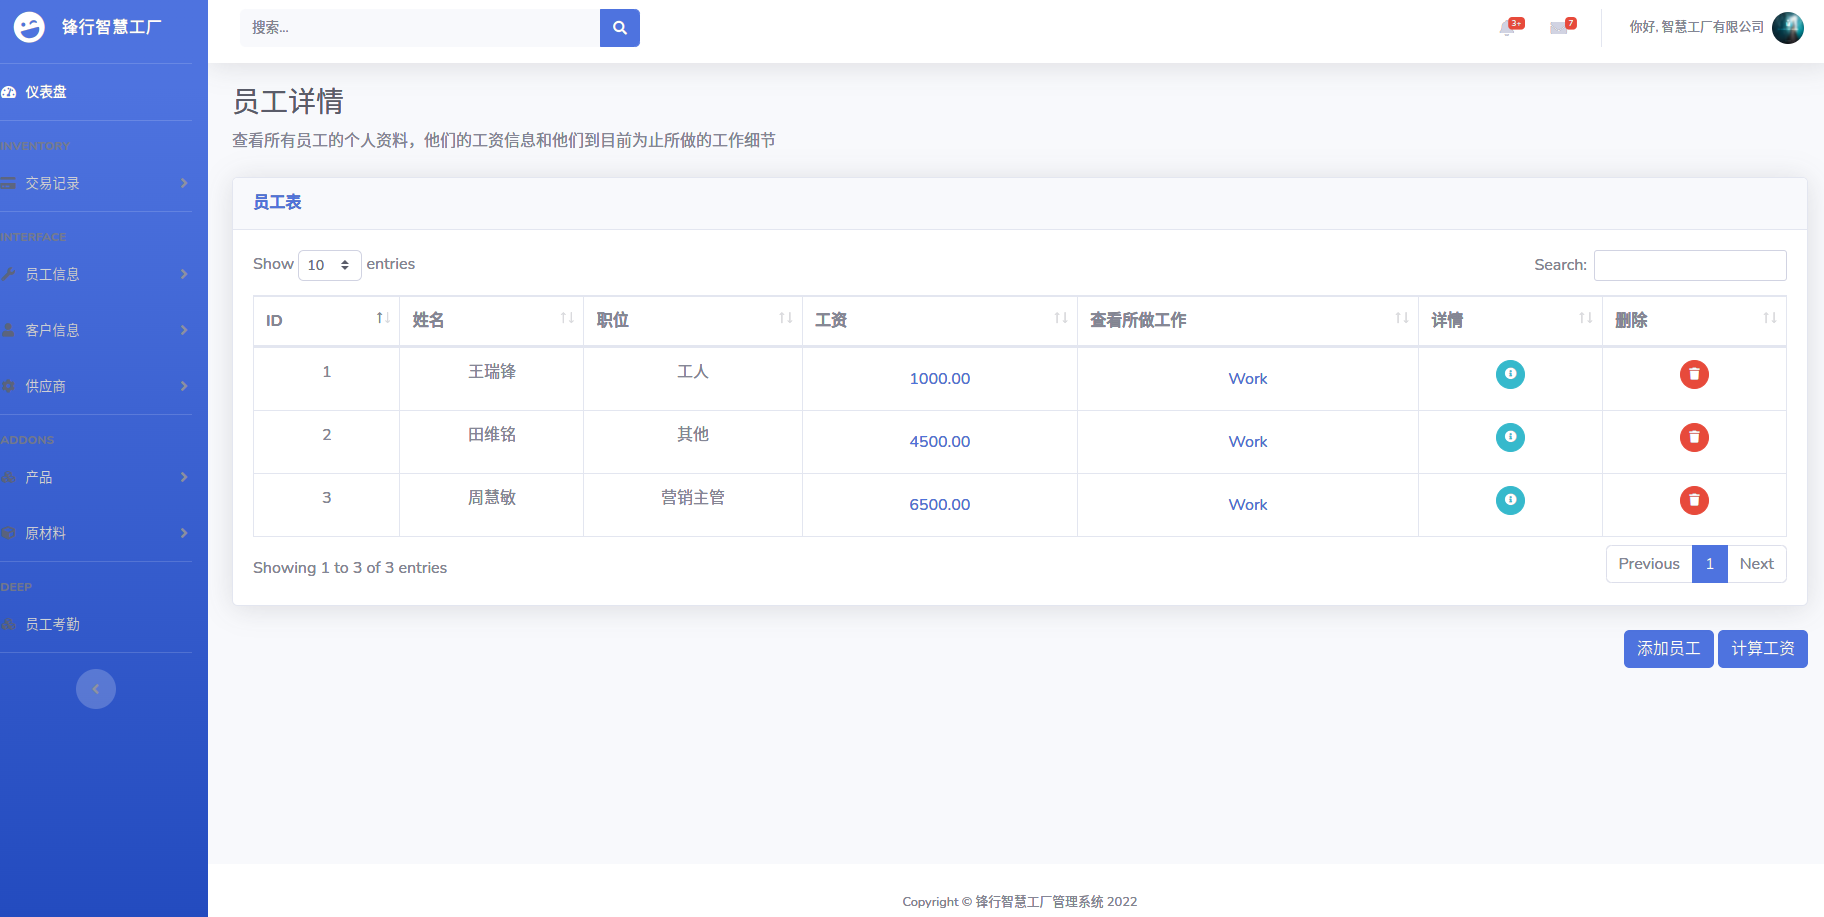
\includegraphics[width=\textwidth]{figures/5employeedetail.png}
        \subcaption{员工信息详情图}
        \label{fig:empledtl}
    \end{subfigure}
    \qquad
    \begin{subfigure}{.45\textwidth}
        \centering
        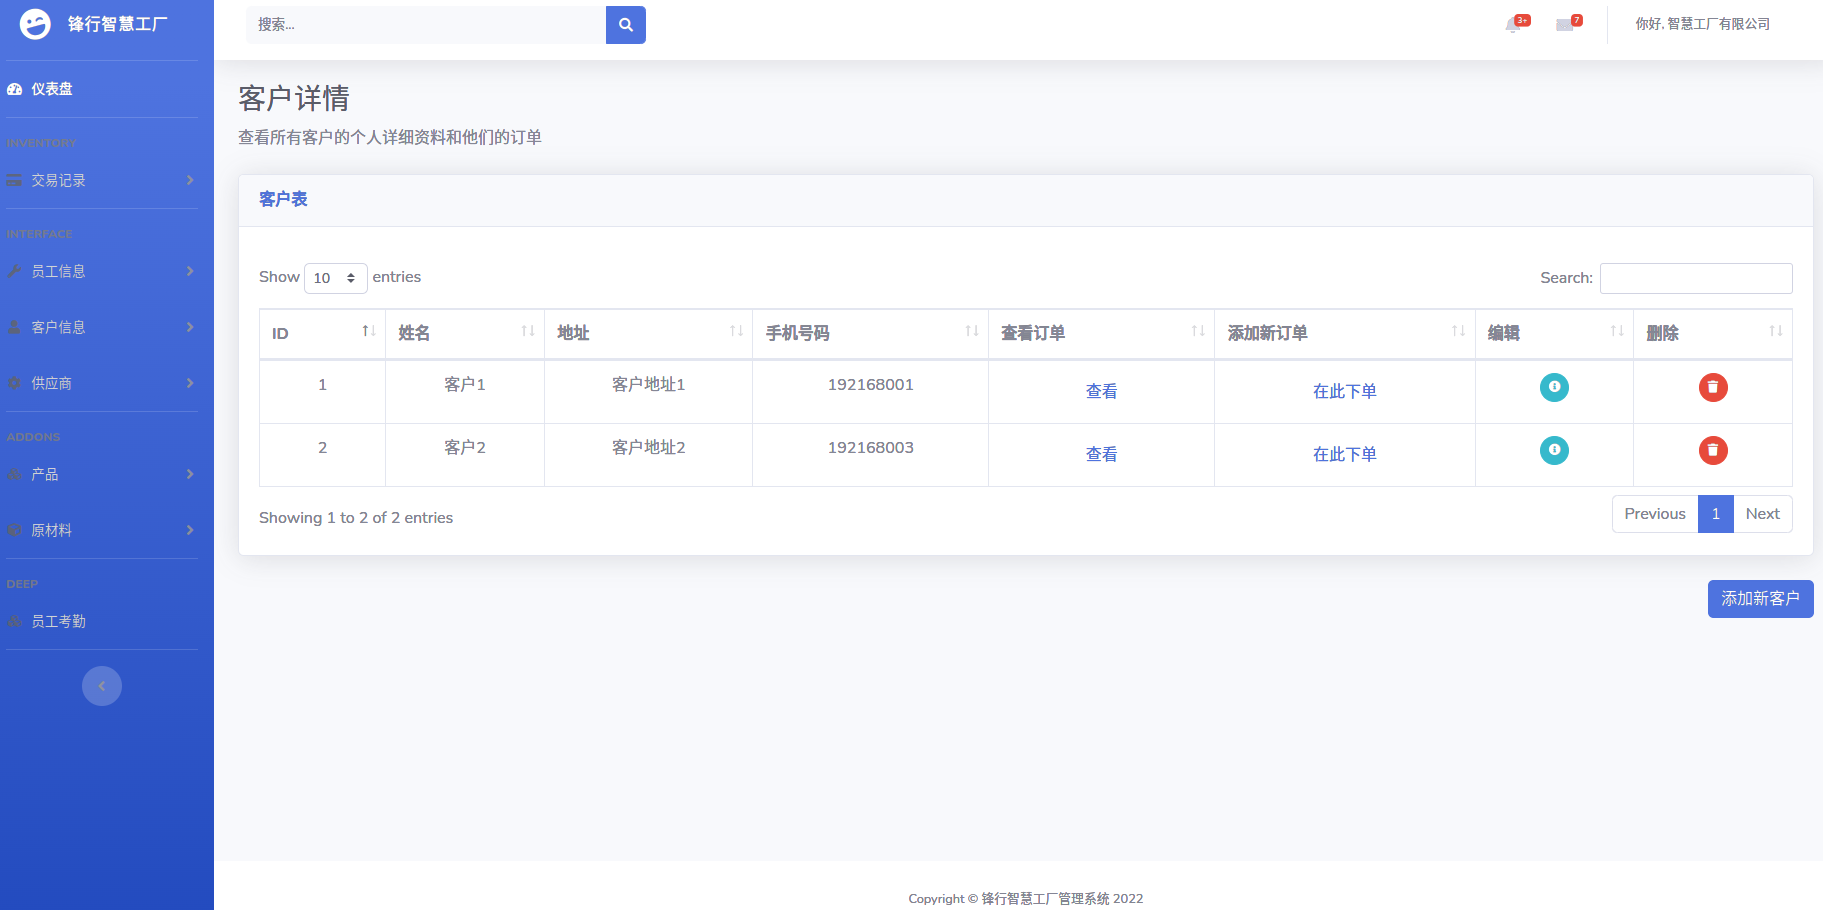
\includegraphics[width=\textwidth]{figures/5customerdetail.png}
        \subcaption{客户信息详情图}
        \label{fig:cstmdtl}
    \end{subfigure}
    \\
    \begin{subfigure}{.45\textwidth}
        \centering
        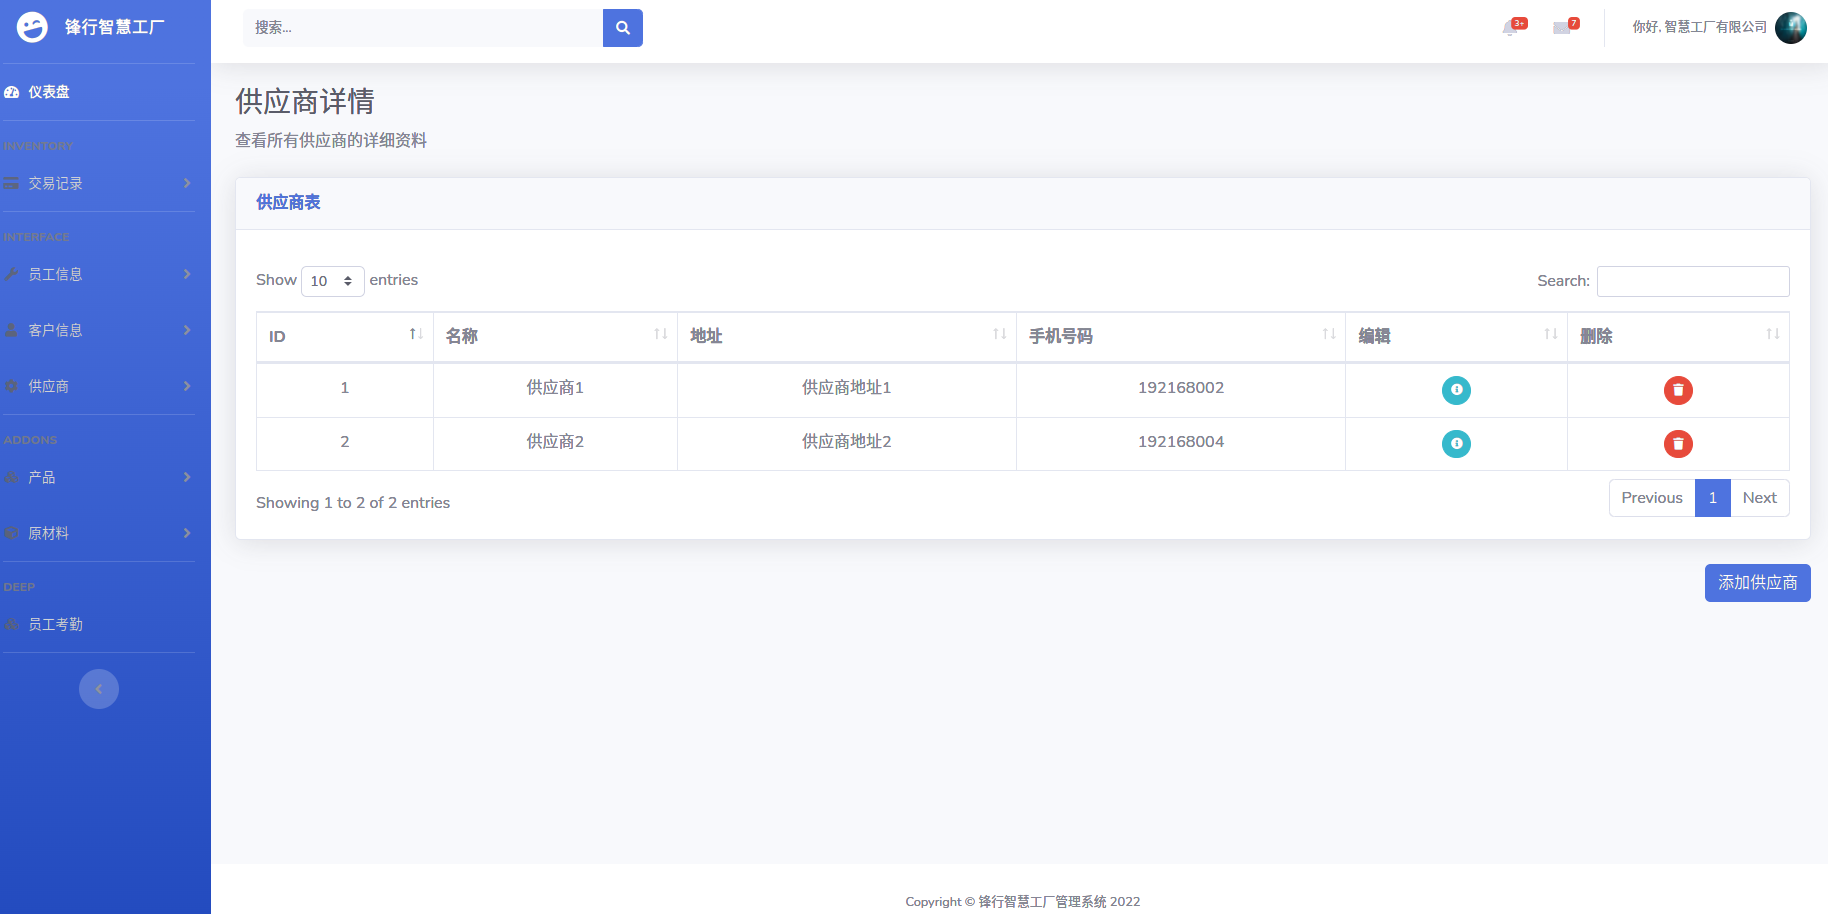
\includegraphics[width=\textwidth]{figures/5supplierdetail.png}
        \subcaption{供应商信息详情图}
        \label{fig:spledtl}
    \end{subfigure}
    \qquad
    \begin{subfigure}{.45\textwidth}
        \centering
        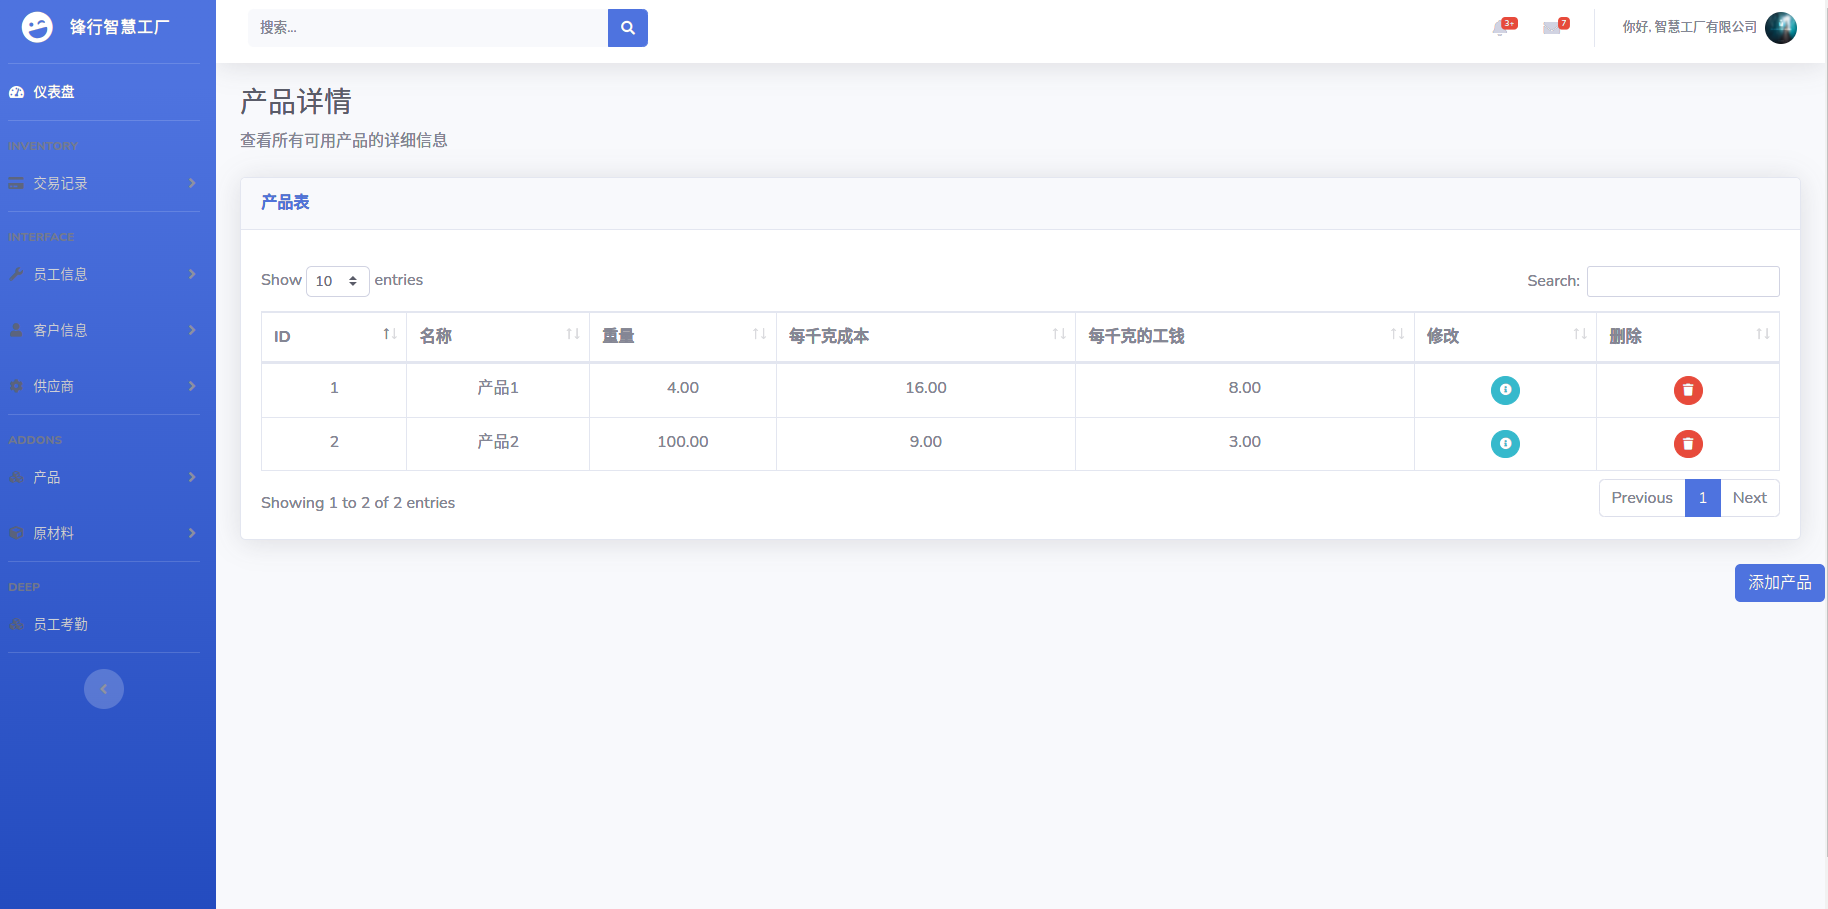
\includegraphics[width=\textwidth]{figures/5productdetail.png}
        \subcaption{产品信息详情图}
        \label{fig:prdctdtl}
    \end{subfigure}
    \caption{后台信息管理详情图图}
\end{figure}

\subsubsection{员工考勤功能实现}

工厂管理员进入到员工考勤页面,向管理员展示一个员工签到记录表,如图\ref{fig:empleatd}所示。并且在上方有一个人脸识别签到的按钮,以供员工以人脸识别的方式进行签到。

\begin{figure}[H]
    \centering
    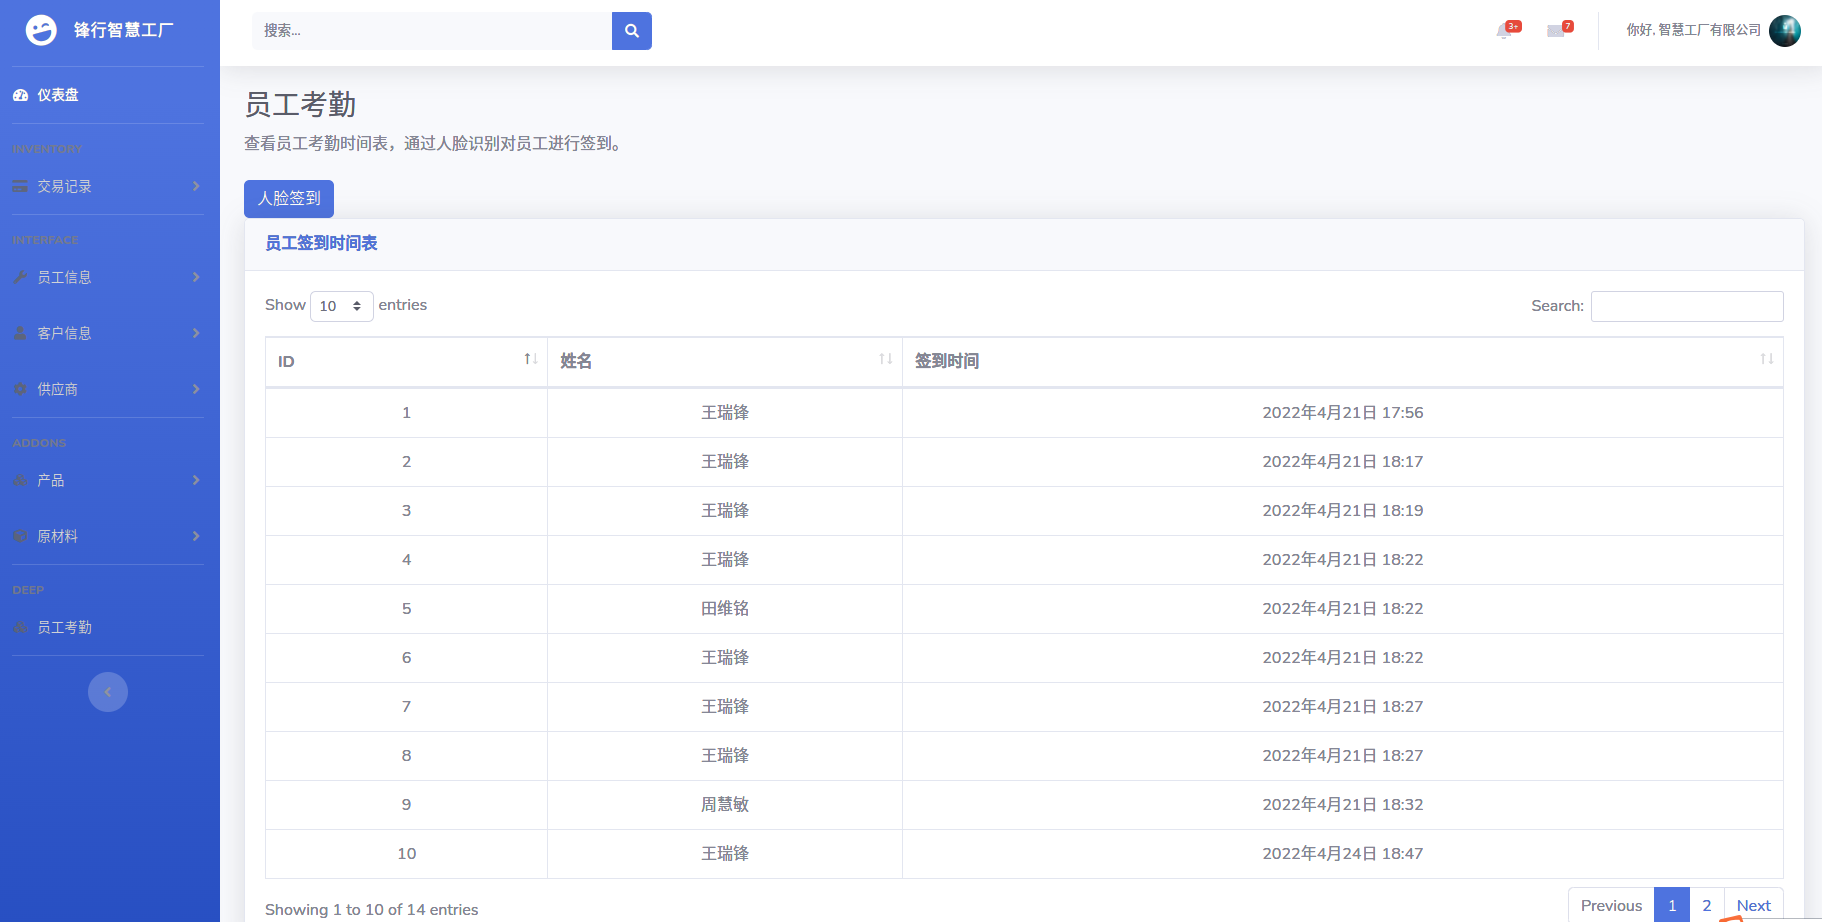
\includegraphics[width=.75\textwidth]{figures/5empleatd.png}
    \caption{员工考勤签到记录详情图}
    \label{fig:empleatd}
\end{figure}

\subsection{人脸识别功能实现}

